
%%%%%%%%%%%%%%%%%%%%%%% file adhocnow15_bolster.tex %%%%%%%%%%%%%%%
%[Ad Hoc Now 2015](http://www.netmode.ntua.gr/adhocnow2015/index.html)
%
%# Dates
%* Deadline: 7/2/15
%* Acceptance: 7/3/15
%* Due: 28/3/15
%* Dates: 29/6/15-2/7/15
%
%# Topics of Interest
%* Access Control 
%* Ad Hoc Networks of Autonomous Intelligent Systems 
%* Algorithmic Issues
%* Analytic Methods and Modeling for Performance Evaluation 
%* Ad Hoc Network Applications and Architectures 
%* Delay-Tolerant Networking
%* Distributed Algorithms for Ad Hoc Networks 
%* Energy Efficiency 
%* Geometric Graphs
%* Location Discovery and Management 
%* Mobility Handling and Utilization 
%* Wireless Mesh Networks
%* Big Data Inspired Data Sensing
%* Mobile Ad Hoc Computing Platforms
%* Systems and Testbeds 
%* Mobile Social Networking 
%* Quality-of-Service 
%* Routing Protocols (Unicast, Multicast, etc.) 
%* Secure Services and Protocols 
%* Sensor Networks 
%* Self-Configuration 
%* Service Discovery 
%* Timing Synchronization 
%* Vehicular Networks 
%* Wireless Internet
%* Processing and Networking Technologies Complexity and Computational Issues
%* Prototype systems and real-world deployment experiences
%
%# Proposed Area of Focus
%Re-present Bellas Chap 4 work with extensions to explain and explore differences between Ad Hoc and Marine.
%
%
%%%%%%%%%%%%%%%%%%%%%%%%%%%%%%%%%%%%%%%%%%%%%%%%%%%%%%%%%%%%%%%%%%%


\documentclass[runningheads,a4paper]{llncs}

\usepackage{amssymb}
\usepackage{amsmath}
\setcounter{tocdepth}{3}
\usepackage{graphicx}

\usepackage{url}
\newcommand{\keywords}[1]{\par\addvspace\baselineskip
\noindent\keywordname\enspace\ignorespaces#1}

\begin{document}

\mainmatter  % start of an individual contribution

% first the title is needed
\title{DRAFT: Trust Framework Operation in Autonomous Marine Communications Environments}
\subtitle{In Preparation for Submission Ad-Hoc Now 2015, Athens, June 29 - July 02 2015. Deadline 07 Feb 2015}

% a short form should be given in case it is too long for the running head
\titlerunning{Trust Framework Operation in Marine Communications Environments}

% the name(s) of the author(s) follow(s) next
%
% NB: Chinese authors should write their first names(s) in front of
% their surnames. This ensures that the names appear correctly in
% the running heads and the author index.
%
\author{Andrew Bolster%
\thanks{Please note that the LNCS Editorial assumes that all authors have used
the western naming convention, with given names preceding surnames. This determines
the structure of the names in the running heads and the author index.}
, Alan Marshall, Ji Guo}
%
\authorrunning{Trust Framework Operation in Marine Communications Environments}
% (feature abused for this document to repeat the title also on left hand pages)

% the affiliations are given next; don't give your e-mail address
% unless you accept that it will be published
\institute{Advanced Networks Research Group, \\Department of Electrical Engineering \& Electronics,\\
University of Liverpool, UK\\
\url{{andrew.bolster,alan.marshall}@liv.ac.uk}\\
\url{http://www.anrg.liv.ac.uk/}}

%%%%%%%%%%%%%%%%%%%%%%%%%%%%%%%%%%%%%%%%%%%%%%%%%%%%%%%%%%%%%%%%%%%%%%%%%%%%%%%%%%%%%%%%%%%%%%
\toctitle{THIS IS JUST FOR KEEPING TRACK OF STRUCTURAL CHANGES IN THE DRAFT}
\tocauthor{IGNORE ME}
\maketitle
\tableofcontents                                                 %DELETE ME BEFORE PUBLICATION
%%%%%%%%%%%%%%%%%%%%%%%%%%%%%%%%%%%%%%%%%%%%%%%%%%%%%%%%%%%%%%%%%%%%%%%%%%%%%%%%%%%%%%%%%%%%%%

%\maketitle                                                   %UNCOMMENT ME BEFORE PUBLICATION

%%%%%%%%%%%%%%%%%%%%%%%%%%%%%%%%%%%%%%%%%%%%%%%%%%%%%%%%%%%%%%%%%%%%%%%%%%%%%%%%%%%%%%%%%%%%%%


\begin{abstract}
  This paper presents a Trust Management Framework (TMF) for Marine Autonomous Networks, including a critique of previous group work in this area utilising Fuzzy Sets and Gray Theory.
  We present a comparative study on the operation and performance of such trust frameworks between the terrestrial and the harsh underwater communications environments. 
  We demonstrate the need for a different approach towards metric selection and trust-timing in such constrained networks. 
\keywords{ad-hoc, MANET, trust, marine, underwater, acoustic}
\end{abstract}

\section{Introduction}\label{sec:introduction}

As mobile ad-hoc networks (MANETs) grow beyond the terrestrial arena, their operation and the protocols designed around them must be reviewed to assess their suitability and optimality in different communications environments to ensure their continued security, reliability, and performance.

Trust Management Frameworks (TMFs) provide information to assist the estimation of future states and operations of nodes within networks. 
This information is used to optimize the performance of a system of systems in the face of malicious, selfish, or defective behavior by one or more nodes within such a system. 
Previous research has established the advantages of implementing distributed TMFs in terrestrial, 802.11 based mobile ad-hoc networks (MANETs), particularly in terms of preventing selfish operation in constrained collaborative systems \cite{Li2007}, and maintaining throughput in the presence of malicious actors \cite{Buchegger2002}

Current TMFs generally use a single type of observed action to derive trust metrics, i.e. successfully forwarded packets. These historical observations then inform future decisions of individual nodes, for example, the selection of a forward router with the lowest previous Packet Loss Rate (PLR) \cite{Li2008}.

Recent work has demonstrated the use of a number of metrics together, forming a ‘vector’ of trust. 
In the case of \cite{Guo2012}, these metrics related to inter-node communications. 
This vectorized trust allows a system to detect anomalous behavior and identify the tactics being used to undermine or subvert trust.

However, this work has been limited to terrestrial, RF based, communications networks.
As Autonomous underwater vehicles (AUVs) become more capable, and economical, they are being used in a many defence, commercial and environmental applications. 
These applications are tending towards utilising  independent collective behaviour of teams or fleets of these platforms \cite{Caiti2011}
With this use being increasingly independent of classical command and control structures, the accurate and timely establishment of mutual and distributed communications trust between nodes within such fleets is essential for the reliability and stability of such systems, and to the secure integration of such systems into larger management systems-of-systems. 

As such, the application of Trust methods developed in the Terrestrial MANET space must be re-appraised for application within the challenging underwater communications channel.

\subsection{Paper Structure}

In section \ref{sec:trustandtmfs} we discuss Trust and Trust Management Frameworks, defining our terminology and reviewing the justifications for the use and development of Trust Management Frameworks. We then review the results presented in \cite{Guo11} and discuss the differences in experimental setup when transitioning to the marine space.
In section \ref{sec:marineacousticnetworks}, we review selected features of the underwater communications channel, highlighting particular challenges and differentials against terrestrial equivalents. 
In section \ref{sec:initialsystemcharacterisation} we establish the initial parameters for simulation and set out a series of experiments to establish commonality between trust establishment in Terrestrial and Marine networks, characterising the communications and physical configuration with respect to the application and channel characteristics.
In section \ref{sec:trustresultsanddiscussion}, we present our findings in trust establishment in this optimal network, pointing out the differences in metric selection and their impact on trust assessment stability.

\subsection{Contributions}
\begin{itemize}
  \item A Trust Management Framework applicable to Underwater MANETs.
  \item A study on the comparitive operation and performance between Terrestrial and Underwater MANETs.
  \item A review of metric suitability for Trust Management Frameworks in Marine Environments, informing future metric selection for experimenters and theorists.
\end{itemize}

\section{Trust and Trust Management Frameworks}\label{sec:trustandtmfs}

\subsection{Trust in MANETs}\label{sec:trustinmanets}

In human trust relationships it can be seen that there can be several perspectives of Trust for example organizational, sociological, interpersonal, psychological and neurological \cite{Lee2004}. 

For the purposes of this work we define two perspectives on trust for autonomous systems: Design and Operational. These are summarised as follows:

\begin{itemize}
  \item \emph{Design Trust}; When an autonomous system is under development a level of Trust is established in it through the manner in which it has been designed and tested. This is the same as conventional systems. The difference with systems that have high-levels of autonomy is that they are designed to behave adaptively to dynamic environments that are difficult to fully predict prior to operational deployment. For example, in a navigation system it is difficult to predict the dynamic environment it will need to adapt to. So Trust needs to be developed that the design and test of such systems are sufficient to predict that operation will be, if not optimal, at least satisfactory.

  \item \emph{Operational Trust}; Trust at runtime or in-situ that both the individual nodes within a system are operating as expected\footnote{Operational Trust is functionally derived from, but distinct from Design Trust}; and that the interfaces between the operator and the system are as expected. This latter aspect covers issues such as physical/wireless links and interpretation of data at each end of such a communication link.
\end{itemize}

In addition to the two perspectives of trust identified, it is necessary to define and classify Operational Trust into two distinct but related sections, which we define as being:
\begin{itemize}
  \item \emph{Hard Trust} or technical trust, being the quantitative measurement and communication of the expectation of an actor performing a certain task, based on historic performance and through consensus building within a networked system. Can be thought of as a de-risking strategy to measure and monitor the ability of a system, or another actor within a system, to perform a task unsupervised.
  \item \emph{Soft Trust} or common trust, being the qualitative assessment of the ability of an actor to perform a task or operation consistently and reliably based on social or experiential factors. This is the ‘natural’ form of trust and is the main motivational driver for the human-factors trust discussion. Can be rephrased as the level of confidence an operator has in an actor to perform a task unsupervised.
\end{itemize} 

% THIS COULD COME IN HANDY LATER % It is already clear that these two definitions are extremely close in their construction, but represent fundamentally different approaches to trust, one coming from a sociological perspective of person-to-person and person-to-group relationships from day to day life, and the other coming from a statistical or formal appraisal of an activity by a system.
For the purposes of this work, we are concerned with the analytical establishment of hard trust within a topologically dynamic network of autonomous actors.

\subsection{Current Trust Management Frameworks}

Various models and algorithms for describing trust and developing trust management in distributed systems, P2P communities or wireless networks have been considered. Taking two examples;

\begin{itemize}
  \item \emph{The Objective Trust Management Framework} takes a Bayesian network approach and introduces the idea of applying a Beta function to changes in the per-link Packet Loss Rate (PLR) over time as an encapsulation method, combining ``Trust'' and ``Confidence of Assessment'' into a single value \cite{Li2008}. 
OTMF however does not appropriately combat multi-node-collusion in the network \cite{Cho2011}. 

  \item \emph{Trust-based Secure Routing \cite{Moe2008a}} demonstrated an extension to Dynamic Source Routing (DSR), incorporating a Hidden Markov Model of the wider ad-hoc network, reducing the efficacy of Byzantine attacks, particularly black-hole attacks but, along with many more TMFs surveyed in \cite{Cho2011}, falls under the same limitation of focusing on single metric observation (PLR). 
  \item \emph{CONFIDANCE}; \textbf{DRAFT: Add \cite{Buchegger2002} in here if there's space, or find something more recent built on it}
\end{itemize}

These single metric TMFs provide malicious actors with a significant advantage if their activity is undetectable by that one assessed metric, especially if the attacker knows the metric in advance. 

The objective of operating a TMF is to increase the confidence in, and efficiency of, a system by reducing the amount of undetectable negative operations an attacker can perform. 
This space of potential attacks can be described as the ‘Threat Surface’. 
In the case where the attacker can subvert the TMF, the metric under assessment by that TMF does not cover the threat mounted by the attacker. 
In turn, this causes a super-linearly negative effect in the efficiency of the network as the TMF is assumed to have reduced the threat surface when in fact it has only made it more advantageous to attack a facet of the networks operation.  
\cite{Huang2010a} also raised the need for a more expanded view of trust but did so with a domain-partitioning approach rather than combining trust assessments from multiple domains within networks. 

\subsection{Grey Relational Trust for Terrestrial MANETs}

\cite{Guo2012} demonstrated the ability of Grey Relational Analysis (GRA)\cite{Zuo1995} to normalize and operationally combine disparate traits of a communications link such as instantaneous throughput, received signal strength, etc. into a single comparable value, a Grey Relational Coefficient, or a ``trust vector''.
This vector is given

\begin{align}
  \label{eq:grc}
  \theta_{k,j}^t = \frac{\min_k|a_{k,j}^t - g_j^t| + \rho \max_k|a_{k,j}^t-g_j^t|}{|a_{k,j}^t-g_j^t| + \rho \max_k|a_{k,j}^t-g_j^t|} \\
  \phi_{k,j}^t = \frac{\min_k|a_{k,j}^t - b_j^t| + \rho \max_k|a_{k,j}^t-b_j^t|}{|a_{k,j}^t-b_j^t| + \rho \max_k|a_{k,j}^t-b_j^t|}
\end{align}

where $a_{k,j}^t$ is the value of a observed metric $j$ for a given node $k$ at time $t$, $\rho$ is a distinguishing coefficient normally set to $0.5$, $g$ and $b$ are respectively the 'good' and 'bad' reference metric sequences from $\{a_{k,j}^t, k=1,2\dots K\}$, e.g. $g_j=\max_k({a_{k,j}^t})$,  $b_j=\min_k({a_{k,j}^t})$ (where each metric is selected to be monotonically increasingly positive for trust assessment, eg Throughput). $\theta$ and $\phi$ are then scaled to $[0,1]$ using the mapping $y = 1.5 x - 0.5$.
The vector natures of $[\theta,\phi]$ allow per-metric weighting before generating a single trust assessment, and also allows the identification and classification of untrustworthy agents.
These weighted $[\theta,\phi]$ values are then condensed into a single trust value by
\begin{equation}
  \label{eq:trustvalue}
  T_k^t = \frac{1}{1+\frac{(\phi_k^t)^2}{(\theta_k^t)^2}}
\end{equation}
For applications involving low fidelity, temporally sparse metrics with unknown statistical distributions, GRA is a more stable comparative analysis, providing an interval of potential trust values rather than fuzzy-logic or the Bayesian-Beta distributions found in current TMFs \cite{Liu2006}. 

GRA, combined with a fuzzy whiteization model \eqref{eq:whitenization}, and a topology-aware weighting scheme \eqref{eq:networkeffects} provide capability to both detect the existence of a malicious agent within the network, and to classify what trust metrics that attacker is manipulating, identifying the style of attack taking place.

There are three classes of topological trust relationship; Direct, Recommendation, and Indirect.
To take the example of a node $n_i$ monitoring the trust of another, target, node, $n_j$; the Direct relationship is simply the trust assessment based on $n_i$'s own observations and experience of $n_j$'s behaviour.
In the Recommendation case, another node, $n_k$, which shares direct relationships with both $n_i$ and $n_j$, gives it's opinion on the trustworthiness of $n_j$ to $n_i$.
The Indirect case is similar to the recommendation case, except that the recommender $n_k$, does not have a (current) direct link with the target $n_j$ but that has a direct link with the observer node, $n_i$.

These relationships give us node sets, $N_R$ and $N_I$ containing the nodes that have recommendation or indirect, relationships to the observing node respectively.

\begin{align}
  \label{eq:whitenization}
  f_1(x) &= -x+1\notag\\
  f_2(x) &= 
  \begin{cases}
    2x & \text{if }x\leq 0.5\\
    -2x+2 & \text{if }x>0.5
  \end{cases}\\
  f_3(x) &= x\notag
\end{align}

\begin{align}
  \label{eq:networkeffects}
  T_{i,j}^{net}=&\frac{1}{2} \cdot \max_s\{f_s(T_{i,j})\} T_{i,j}&\qquad \text{Direct Trust}\notag \\
  &+ \frac{|N_R| }{2|N_R| + |N_I|}\sum_{n \in N_R} \max_s\{f_s(T_{i,n})\} T_{i,n}&\qquad \text{Recommendation Trust}\notag\\
  &+ \frac{|N_I| }{2|N_R| + |N_I|}\sum_{n \in N_I} \max_s\{f_s(T_{i,n})\} T_{i,n} &\qquad \text{Indirect Trust}
\end{align}

\cite{Guo11} demonstrated the stochastic variation of this methodology wrt. attack method, enabling the detection and identification of the aspect of network operation under attack.
It is this work that is being expanded upon in paper.

\subsection{Scenarios}

Four Mobility scenarios were used in \cite{Guo11} to explore the trust-behaviour, covering the majority of MANET operational requirements; 

\begin{itemize}
  \item All Nodes Static
  \item Central node performing a random walk with leaf-nodes static
  \item Leaf-nodes randomly walking with central node static
  \item All nodes randomly walking
\end{itemize}

The six nodes were arranged in the form of a flattened pentagon with the 'central' node ($n_1$) placed near the geometric middle, such that each node was on average 100m from its neighbours.

In all of the scenarios, each link from $n_i \rightarrow n_j$ sent a 10 second of Constant Bit Rate (CBR) style traffic.

\begin{figure}[h]
  \centering
  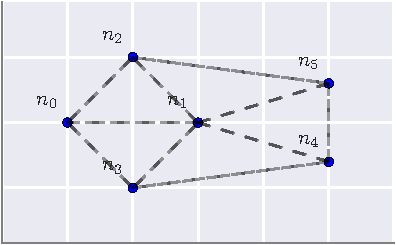
\includegraphics[width=0.45\textwidth]{img/s1_layout.pdf}
  \caption{Initial Scenario Topology, with nodes spaced an average of 100m apart}
  \label{fig:s1_layout}
\end{figure}

\section{Marine Acoustic Networks}\label{sec:marineacousticnetworks}

The key challenges of underwater acoustic communications are centred around the impact of slow and differential propagation of energy (RF, Optical, Acoustic) through water, and it's interfaces with the seabed / air.
The resultant challenges include; long delays due to propagation, significant inter-symbol interference and Doppler spreading, fast and slow fading due to environmental effects (aquatic flora/fauna; surface weather), carrier-frequency dependent signal attenuation, multipath caused by the medium interfaces at the surface and seabed, variations in propagation speed due to depth dependant effects (salinity, temperature, pressure, gaseous concentrations and bubbling), and subsequent refractive spreading and lensing due to that same propagation variation.\cite{Partan2006}

The attenuation that occurs in an underwater acoustic channel over a distance $d$ for a signal about frequency $f$ in linear and $dB$ forms respectively is given by

\begin{equation}
  \label{eq:acoattenuation}
  A(d,f) = A_0d^ka(f)^d
\end{equation}
\begin{equation}
  \label{eq:acoattenuationdb}
  10 \log A(d,f)/A_0 = k \cdot 10 \log d + d \cdot 10 \log a(f)
\end{equation}

where $A_0$ is a unit-normalising constant, $k$ is a spreading factor (commonly taken as 1.5), and $a(f)$ is the absorption coefficient, expressed empirically using Thorp's formula \eqref{eq:thorp} from \cite{Stojanovic2007}

\begin{equation}
  \label{eq:thorp}
  10 \log a(f) = 0.11 \cdot \frac{f^2}{1+f^2} + 44\cdot\frac{f^2}{4100+f^2}+ 2.75\times10^{-4} f^2 + 0.003
\end{equation}


Thus, the multi-path channel transfer function can be described by 

\begin{equation}
  \label{eq:acomultipath}
  H(d,f) =\sum_{p=0}^{P-1} h(p) = \sum_{p=0}^{P-1} \Gamma_p / \sqrt{A(d_p,f)}e^{-j 2 \pi f \tau_p}
\end{equation}

where $d=d_0$ is the minimal path length between the transmitter and receiver, $d_p,p=\{1,\dots P-1\}$ are the secondary path lengths, $\Gamma_p$ models additional losses incurred on each path such as reflection losses at the surface interface, and $\tau_p = d_p/c$ is the delay time ($c = 1500 ms^{-1}$ is the nominal speed of sound underwater).


This combination of refractive lensing and the multipath nature of the medium result in supposedly ``line of sight'' propagation being extremely unreliable for estimating distances to targets, as the first arriving beam has as the very least bent in the medium, and commonly has bounced between the surface/seabed before arriving at a receiver. Further, this affect is usually anisotropic with differential depths between transmitter and receiver, meaning that any variation in depth across a channel, greatly impacts the characteristics of that channel.

Comparing \eqref{eq:acoattenuation} with the RF Free-Space Path Loss model \eqref{eq:fspl}, while both are frequency and distance dependant; 

\begin{equation}
  \label{eq:fspl}
  A_{rf}(d,f) \approx \left( \frac{4\pi f}{c} \right)^2
  \text{where }c\approx 3\times10^8m/s
\end{equation}



\subsection{Trust Requirement in Marine Networks}

In this subsection we establish the requirement for communications trust in acoustic marine networks, extending and expanding on the generic assessment given in \ref{sec:trustinmanets}

\section{Initial System Model Characterisation}\label{sec:initialsystemcharacterisation}

\subsection{Simulation Background}

Simulations were conducted using a Python based agent simulation framework based on SimPy\cite{Mueller2003SimPy}, with a network stack built upon the AUVNetSim stack\cite{Miquel2008}, with transmission parameters taken from and validated against \cite{Stojanovic2007} and \cite{Stefanov2011}.

Given the differences in delay and propagation between RF and marine networks, it is natural that the same application rates (e.g. packet emission rates or throughput) cannot be maintained under such different constraints. 
Therefore, before we can fairly assess the trust operation of a Underwater MANET, we first establish it's operational characteristics. 

Specifically, we sought to define a methodology for establishing a near-optimal operation point. This was done in two parts; optimisation for network level queuing, optimisation for physical layout scaling.

\begin{table}[h]
  \caption{Comparison of system model constraints as applied between Terrestrial and Marine communications} \label{tab:sysconstraints}
  \begin{center}
    \setlength{\tabcolsep}{8pt}
    \begin{tabular}{|l|c|c|c|}
      \hline
      Parameter & Unit & Terrestrial & Marine \\
      \hline
      Simulated Duration & $s$ & 300 & 36000\\
      Simulated Area & $km^2$ & 0.7 & 0.7 \\
      Transmission Range & $km$ & 0.25 & 1.5 \\
      Number of Nodes & & 6 & 6 \\
      Comms Medium & & RF(802.11) & Acoustic\\
      MAC Type & & CSMA/CA & CSMA/CA\\
      Propagation Speed& $m/s$ & $3\times10^8$ & 1490\\
      Center Frequency& $Hz$ & $2.6\times10^9$ & $10^3$ \\
      Bandwidth& $Hz$ & $22\times10^6$ & $10^3$\\
      Routing Protocol & & DSDV & FBR \\
      Mobility & & Various & Various \\
      Max Speed & $ms^{-1}$ & 5 & 1.25 \\
      Data Rate & $bps$ & $10^6$ & 240 \\
      Burst Counts & & 10 & 1 \\
      Packet Size & bits & 4096 & 9600 \\
      Destination Selection & & Random & Random\\
      Single Transmission Duration & $s$ & 10 & 32 \\
      Single Transmission Size & bits & $10^7$ & $9600$ \\
      \hline
    \end{tabular}
    \setlength{\tabcolsep}{6pt}
  \end{center}
\end{table}


\subsection{Establishing Scale Factors in Communications Rate}

In this section we characterise the simulated communications environment, establishing an optimal packet emission rate for comparison against \cite{Guo11}. 

This is pretty much summarised in\ref{fig:throughput_performance_static} and \ref{fig:prod_breakdown} 

\begin{figure}[h]
  \centering
  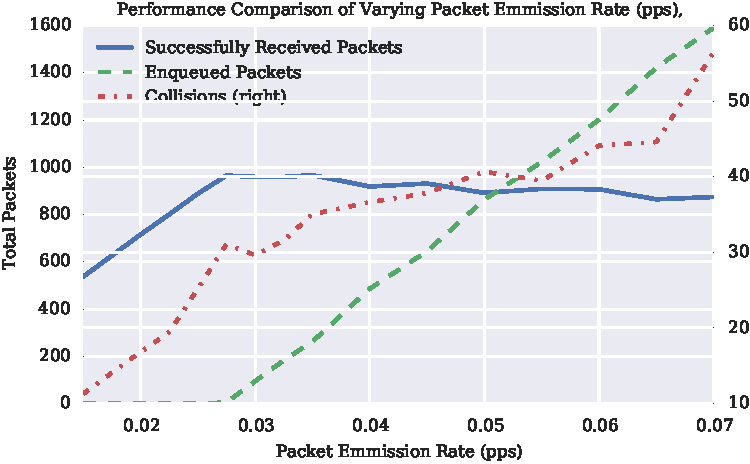
\includegraphics[width=0.6\textwidth]{img/throughput_performance_static.pdf}
  \caption{Varying packet emission rate demonstrates maximal throughput at 0.025 packets per second, equivalent to $\approx$240 bps}
  \label{fig:throughput_performance_static}
\end{figure}


\begin{figure}[h]
  \centering
  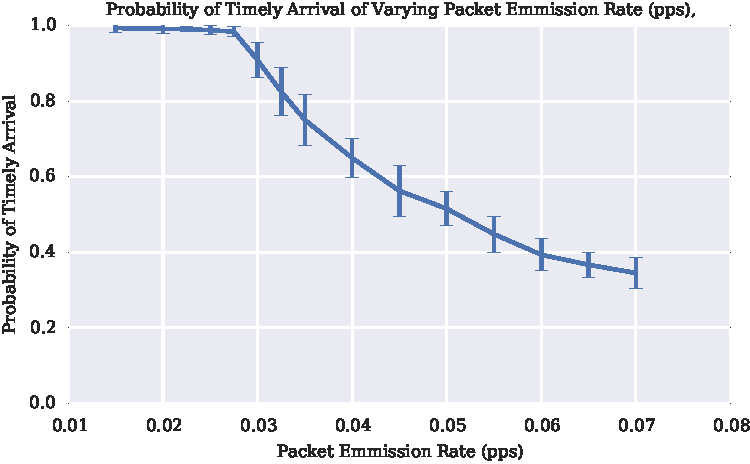
\includegraphics[width=0.6\textwidth]{img/prod_breakdown_static.pdf}
  \caption{Varying packet emission rate demonstrates a saturation point at 0.025 packets per second}
  \label{fig:prod_breakdown}
\end{figure}


\subsection{Establishing Scale Factors in Physical Distribution}

In this section we characterise the simulated communications environment, establishing an optimal node-separation scaling for comparison against \cite{Guo11}
This is pretty much summed up below.
\begin{figure}[h]
  \centering
  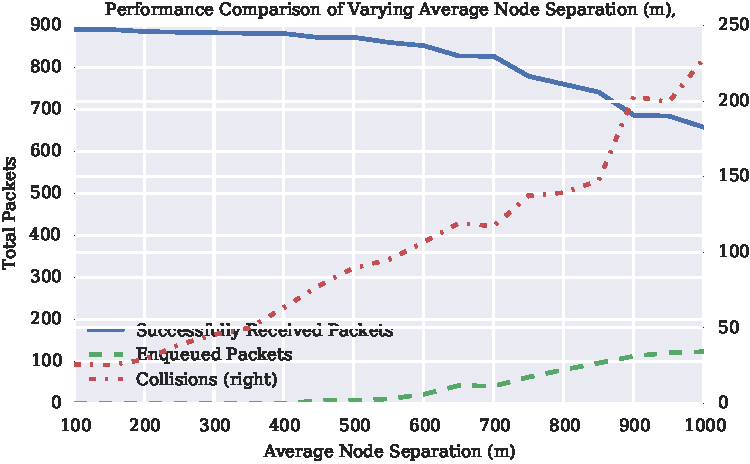
\includegraphics[width=0.6\textwidth]{img/throughput_performance_range.pdf}
  \caption{Varying average node separation shows that while direct throughput isn't affected, collision rates are. However, this collision rate is well within the tolerances of the MAC layer}
  \label{fig:throughput_performance}
\end{figure}

It may be worth going back to the range scaling experiments to effectively do a ``square'' study; establishing the breakdown points for each scale, but that's for after this.


\subsubsection*{Acknowledgments.} The heading should be treated as a
subsubsection heading and should not be assigned a number.

\section{The References Section}\label{references}

%\bibliographystyle{amsplain} % UNCOMMENT BEFORE PUB!!!!!!!!!!!!!!!!!!!!!!!!!!!!!!!!!!!!!!!!!!!!!!1
\bibliographystyle{apalike}
\bibliography{refs}
% 
% \begin{thebibliography}{4}
% 
% \bibitem{jour} Smith, T.F., Waterman, M.S.: Identification of Common Molecular
% Subsequences. J. Mol. Biol. 147, 195--197 (1981)
% 
% \bibitem{lncschap} May, P., Ehrlich, H.C., Steinke, T.: ZIB Structure Prediction Pipeline:
% Composing a Complex Biological Workflow through Web Services. In: Nagel,
% W.E., Walter, W.V., Lehner, W. (eds.) Euro-Par 2006. LNCS, vol. 4128,
% pp. 1148--1158. Springer, Heidelberg (2006)
% 
% \bibitem{book} Foster, I., Kesselman, C.: The Grid: Blueprint for a New Computing
% Infrastructure. Morgan Kaufmann, San Francisco (1999)
% 
% \bibitem{proceeding1} Czajkowski, K., Fitzgerald, S., Foster, I., Kesselman, C.: Grid
% Information Services for Distributed Resource Sharing. In: 10th IEEE
% International Symposium on High Performance Distributed Computing, pp.
% 181--184. IEEE Press, New York (2001)
% 
% \bibitem{proceeding2} Foster, I., Kesselman, C., Nick, J., Tuecke, S.: The Physiology of the
% Grid: an Open Grid Services Architecture for Distributed Systems
% Integration. Technical report, Global Grid Forum (2002)
% 
% \bibitem{url} National Center for Biotechnology Information, \url{http://www.ncbi.nlm.nih.gov}
% 
% \end{thebibliography}

\end{document}
